% !TeX root = ../main.tex
\chapter{理论设计}  
由于四旋翼的推力方向只能向下,因此无法在不倾斜的情况下获得水平方向的推力从而改变水平位置。因此刚体的六个自由度无法同时被控制,使得四旋翼欠驱动,输入的维度是4,所以能直接控制的状态维度也是4。虽然四旋翼整体并不满足高阶全驱系统理论的要求,但是姿态环的三个自由度是全驱的,这从式\ref{equ:M}\ref{equ:dotR}可以清楚得看到。

四旋翼的控制分为姿态环和位置环两部分。从物理原理角度,分模态讨论,水平面内的飞行是对称的,以向前飞为例,需要机身先向前倾斜才能获得向前的分力。因此姿态的变化先于位置的变化,在实践中,姿态环的控制频率也远大于位置环。姿态环的动力学方程涉及到更强的非线性,并且姿态环一旦能迅速地达到期望值,位置控制也就水到渠成,因此四旋翼的控制中姿态环的重要性和难度都高于位置环。

\section{姿态控制}

\subsection*{误差定义}
姿态控制采用基于高阶全驱系统理论的方法,那么首先就需要定义一个合适的三维误差向量来描述当前姿态$R$到期望姿态$R_d$的差,使得控制输入矩阵可逆:
\begin{equation}
    e=(R_d^TR-R^TR_d)^\vee
\end{equation}

该误差定义不仅可以满足高阶全驱系统理论的要求,并且如式\ref{error}所示,具有良好的物理意义。当$e\to 0$时,$\theta \to 0$,$R$与$R_d$重合,达到期望。

\subsection*{HOFA模型}
接下来需要对误差连续两次求导,使得方程中出现控制输入,也就是力矩$M$:
$$\begin{aligned}
    \dot e=&[(R_d^TR \Omega-\Omega_dR_d^TR)-(R_d^TR \Omega-\Omega_dR_d^TR)^T]^\vee\\
    =&[R_d^TR(\Omega-R^TR_d \Omega_dR_d^TR)-(R_d^TR(\Omega-R^TR_d \Omega_dR_d^TR))^T]^\vee \\
    =&[R' \hat e_\Omega  + \hat e_\Omega R'^T]^\vee
\end{aligned} $$
    定义
    $$R'=R_d^TR \quad e_\Omega=\omega -R^TR_d \omega_d$$
进一步求二阶导:
    $$\begin{aligned}
        \ddot e =& [(R' \hat e_\Omega \Omega + R'\dot \Omega -\Omega_d R' \hat e_\Omega -\dot \Omega_d R')-(R' \hat e_\Omega \Omega + R'\dot \Omega -\Omega_d R' \hat e_\Omega -\dot \Omega_d R')^T]^\vee\\
        =&[(R' \hat e_\Omega \Omega  -\Omega_d R' \hat e_\Omega -\dot \Omega_d R')-(R' \hat e_\Omega \Omega  -\Omega_d R' \hat e_\Omega -\dot \Omega_d R')^T]^\vee+[R'\dot \Omega-(R'\dot \Omega)^T]^\vee\\
        =&A_d+ \begin{Bmatrix}
        \begin{bmatrix}
        R'_{11} &R'_{12}  & R'_{13} \\
        R'_{21} & R'_{22} & R'_{23} \\
        R'_{31} & R'_{32} &R'_{33}  \\
        \end{bmatrix}&\begin{bmatrix}
        0 & -\dot\omega_3 &\dot\omega_2  \\
         \dot\omega_3& 0 &  -\dot\omega_1\\
         -\dot\omega_2&\dot\omega_1  & 0 \\
        \end{bmatrix}\end{Bmatrix}^\vee -\begin{Bmatrix}
        \begin{bmatrix}
        R'_{11} &R'_{12}  & R'_{13} \\
        R'_{21} & R'_{22} & R'_{23} \\
        R'_{31} & R'_{32} &R'_{33}  \\
        \end{bmatrix}&\begin{bmatrix}
        0 & -\dot\omega_3 &\dot\omega_2  \\
         \dot\omega_3& 0 &  -\dot\omega_1\\
         -\dot\omega_2&\dot\omega_1  & 0 \\
        \end{bmatrix}\end{Bmatrix}^{T\vee}\\
        =&A_d+\begin{bmatrix}
        R'_{22}+R'_{33} & -R'_{21} & -R'_{31} \\
         -R'_{12}& R'_{11}+R'_{33} & -R'_{32} \\
         -R'_{13}&- R'_{23} & R'_{11}+R'_{22} \\
        \end{bmatrix}\dot \omega\\
        =&A_d+R_B\dot \omega
        \end{aligned}  $$

        $$A_d=[(R' \hat e_\Omega \Omega  -\Omega_d R' \hat e_\Omega -\dot \Omega_d R')-(R' \hat e_\Omega \Omega  -\Omega_d R' \hat e_\Omega -\dot \Omega_d R')^T]^\vee$$

        $$R_B=\begin{bmatrix}
            R'_{22}+R'_{33} & -R'_{21} & -R'_{31} \\
             -R'_{12}& R'_{11}+R'_{33} & -R'_{32} \\
             -R'_{13}&- R'_{23} & R'_{11}+R'_{22} \\
            \end{bmatrix}$$
\textbf{$R_B$满秩}

    当$R_B$满秩时,符合高阶全驱的条件;不满秩时则短暂采用替补控制律。代入\ref{equ:M},得:
    $$\begin{aligned}
        \ddot e=&A_d+R_B J^{-1}(-\omega \times J\omega+M)\\
        =&A_d-B \omega\times J\omega +BM
        \end{aligned}$$
        $$B=R_BJ^{-1}$$

    高阶全驱系统建模完成,随即立刻可以设计控制算法。由于$B$可逆,令:
    $$M=-B^{-1} A_d+\omega \times J\omega +B^{-1}M^*$$
    得
    $$\ddot e=M^*$$

    对于该补偿掉所有非线性部分的二阶积分器模型,得到状态空间表示下的方程:
    $$\dot x=\begin{bmatrix}
        0_{3\times 3} & I_{3\times 3} \\
        0_{3\times 3} & 0_{3\times 3}
    \end{bmatrix} x+\begin{bmatrix}
        0_{3\times 3} \\ I_{3\times 3}
    \end{bmatrix} M^* $$
    $$x=\begin{bmatrix}
        e \\ \dot e
    \end{bmatrix}$$
    在此基础上可以便利地采用任何线性系统控制器设计方法,采用LQR控制器,得到$M^*=-kx$

   $$ \begin{aligned}
        M=&-J R_B^{-1} [(R' \hat e_\Omega \Omega  -\Omega_d R' \hat e_\Omega -\dot \Omega_d R')-(R' \hat e_\Omega \Omega  -\Omega_d R' \hat e_\Omega -\dot \Omega_d R')^T]^\vee \\
         &+\omega \times J\omega + J R_B^{-1}(-kx)
    \end{aligned}$$

    \textbf{$R_B$不满秩}

    $R_B$不满秩时,上述高阶全驱方法就不在成立,但是不满秩的点在$\mathbb{R^{3 \times 3}}$是无处稠密的,因此在实验中几乎不会遇到。但是为了理论的完备,设置替补控制律\cite{Lee2010}:
    $$M=-k_R e_R-k_\omega e_\omega+\omega \times J \omega -J(\Omega R'^T \omega_d-R'^T \dot \omega_d) $$
    $$ e_R=\frac{1}{2} (R'-R'^T)^\vee $$
    这种控制律能保证指数收敛,参数$k_R,k_\omega$需要根据转动惯量调试后选定。
    \section{位置控制}
    在设计位置环的控制算法时,首先要结合期望偏航角生成期望姿态$R_d$作为姿态环的输入。然后,考虑到姿态环的高响应速度,其动态过程可以被忽略。这一假设进一步简化了位置环的动力学方程,使其也能被视作一个线性系统,仍然先采用LQR方法进行控制。

    
    \subsection{期望姿态生成}
    期望姿态$R_d$是由位置环输出以及期望偏航角生成的,它代表了要达到期望的位置所需的推力方向。由于无人机的推力只能垂直于机身平面,要到达期望的位置需要有指向该位置的力,因此要首先改变无人机姿态使其法线方向平行于期望推力方向,再结合外部输入的期望偏航角,就能得出期望的姿态\cite{Lee2010}。

    在本课题中,机头的指向即偏航角相对来说没有期望位置重要,且在姿态较大时,偏航角的意义实质上并不明确:偏航角如果是Z-Y-X欧拉角定义下的第一个转角,当后两个转角较大时,偏航角也就脱离了原本的物理意义。因此首先保证期望推力方向,将其设计成反馈加前馈的形式:
    $$f_{ideal}=k_x e_x+k_v e_v-mg \vec e_3+m a_d$$
    $$\vec b_{3d}=-\frac{f_{ideal}}{||f_{ideal}||}$$
    $$ e_x=x_d-x \quad e_v=v_d-v \quad \vec e_3=\begin{matrix}
        [0 & 0 & 1]
    \end{matrix}^T$$

    然后将期望偏航角产生的单位向量$\begin{matrix} [\cos{\psi_d} & \sin{\psi_d} & 0]  \end{matrix}^T$投影到垂直于$b_{3d}$的平面上,就能得到期望姿态$R_d= \begin{matrix} [ \vec b_{2d}\times \vec b_{3d} &\vec b_{2d} & \vec b_{3d}] \end{matrix}$,$\vec b_{2d}=\vec b_{3d} \times \vec b_{1d}$,如图 \ref{fig:2}。
    \begin{figure}[!h]
        \centering
        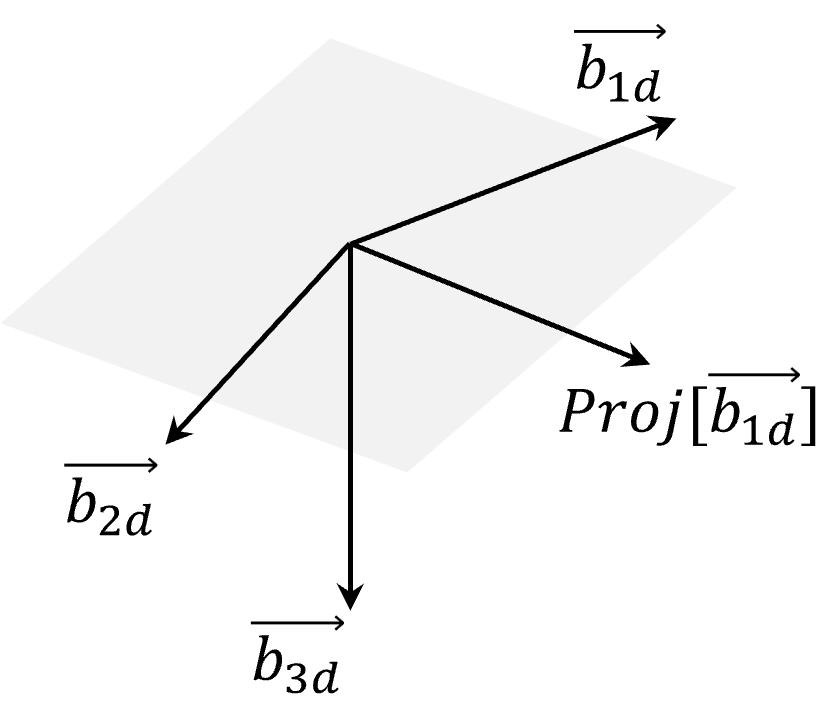
\includegraphics[width=0.3\textwidth]{desired R.png}
        \caption{期望姿态定义}
        \label{fig:2}
      \end{figure}

      \subsection{推力控制律}
      以上计算得到的$f_{ideal}$完全没有考虑姿态动态过程,由于$R$不可能瞬间收敛到$R_d$,当姿态尚未收敛时,推力的控制指令应当为$f_{ideal}$在当前姿态推力方向上的投影,否则会在错误的方向上投入过多的力分量:
      $$f=f_{ideal}\cdot R e_3$$
      接下来需要得出控制律$k_x \quad k_v$,当姿态$R$能迅速收敛到$R_d$时,动力学方程\ref{equ:a}退化为:
      $$m \dot v=mge_3-f$$

      那么位置控制环节就变成了简单的线性系统,可以写作六阶状态空间表示
      $$\dot x=\begin{bmatrix}
        0_{3\times 3} & I_{3\times 3} \\
        0_{3\times 3} & 0_{3\times 3}
    \end{bmatrix} x+\begin{bmatrix}
        0_{3\times 3} \\ \frac{1}{m} I_{3\times 3}
    \end{bmatrix} f +\begin{bmatrix}
        0_{3 \times 1} \\ a_d-g \vec e_3 
    \end{bmatrix}$$
    $$x=\begin{bmatrix}
        x_d -x \\ v_d -v
    \end{bmatrix}$$
      将$f$写作补偿掉前馈的形式:$f=f^*-mg \vec e_3 +m a_d$。接下来就可以运用LQR方法得到控制律$f^*=-kx$。

    $f^*$的控制律并不是四旋翼运动控制的关键,只要期望姿态生成合理并且姿态环能迅速收敛,位置环的控制难度很低。因此在后面的ros仿真以及实机实验中,位置环将不对PX4的代码做更改(PX4的位置环控制算法事实上完全包含了上述算法,将I和D置0即可退化为本文中的方法),以避免架构上不必要的麻烦。
